\documentclass{acm_proc_article-sp}
\usepackage{hyperref}
\usepackage{ngerman}
\usepackage{graphics}
\usepackage{float}
\usepackage{colortbl}
\usepackage{amsmath}
\hypersetup{
    pdftitle={Complex Event Processing am Beispiel von Esper },
    pdfauthor={Martin Steinbach},
    pdfkeywords={Seminar, Rostock, WiSe 2018, 2018},
    pdfsubject={Seminar Event Driven Programming},
    pdfcreator={Martin Steinbach},
    citecolor=blue,
    hypertexnames=false,
    %linktocpage,
    pdfpagelabels,
    plainpages=false,
    backref,
    urlcolor=blue,
    menucolor=red,
    linkcolor=black,
    colorlinks=true,
    bookmarksnumbered,
    %pdffitwindow
}
%\hyphenation{
 
%}
\definecolor{shadecolor}{gray}{.92}
\begin{document}


\title{Complex Event Processing am Beispiel von Esper}
\numberofauthors{1} 
\author{
\alignauthor
Martin Steinbach\vspace{0.1cm}\\
       \affaddr{Institut für Informatik}\\
       \affaddr{Universität Rostock}\\
       %\affaddr{Rostock, Deustchland}\\
       \email{\footnotesize martin.steinbach@uni-rostock.de}}


\maketitle

\begin{abstract}
    \vspace{0.1cm}
\begin{itemize}
    \item steige steigerung der Datenmengen -> keine speicherung möglich
    \item kostengünstige Sensortechnik 
\end{itemize}
lorem ipsum lorem ipsum loren ipsum lorem ipsum lorem \\
lorem ipsum lorem ipsum loren ipsum lorem ipsum lorem \\
lorem ipsum lorem ipsum loren ipsum lorem ipsum lorem \\
lorem ipsum lorem ipsum loren ipsum lorem ipsum lorem \\
lorem ipsum lorem ipsum loren ipsum lorem ipsum lorem \\
lorem ipsum lorem ipsum loren ipsum lorem ipsum lorem \\
lorem ipsum lorem ipsum loren ipsum lorem ipsum lorem \\
lorem ipsum lorem ipsum loren ipsum lorem ipsum lorem \\
lorem ipsum lorem ipsum loren ipsum lorem ipsum lorem \\
lorem ipsum lorem ipsum loren ipsum lorem ipsum lorem \\
lorem ipsum lorem ipsum loren ipsum lorem ipsum lorem \\
lorem ipsum lorem ipsum loren ipsum lorem ipsum lorem \\
lorem ipsum lorem ipsum loren ipsum lorem ipsum lorem \\
lorem ipsum lorem ipsum loren ipsum lorem ipsum lorem \\
lorem ipsum lorem ipsum loren ipsum lorem ipsum lorem \\
\end{abstract}

%\terms{Theory}

\keywords{EDA, CEP, Esper} % NOT required for Proceedings

\section{Einleitung}
\vspace{0.1cm}
Jede Aktion in der IT-gestützten Welt erzeugt 
Informationen in Form von Daten. Dabei spielt es keine Rolle ob ein Verweis in einem 
sozialen Netzwerk verwendet wird, ob ein Sensor einen Messwert meldet, oder jemand eine 
Aktie kauft. Betrachtet man diese Daten, scheint der Informationsgehalt gering und die 
Datenmenge überschaubar. Aus diesen Grund lässt sich aus diesen Einzelinformationen kaum 
eine nutzbringende Auskunft für ein Gesamtsystem konstruieren. In der Praxis relevante
Fragestellungen wären zum Beispiel: Wie oft wird ein Verweis innerhalb einer Zeitspanne 
ausgelöst und zu welcher Tageszeit hauptsächlich? Wie viele Messwerte eines Sensors 
werden benötigt um konkrete Aussagen zu einem Messobjekt machen zu können? Wann und 
welche Menge an Aktien eines Unternehmens werden über einen Zeitraum erworben, 
beziehungsweise verkauft?\\
Um diese exemplarischen Fragen zu beantworten steigt die Anzahl der benötigten Daten sehr 
schnell an und eine Verarbeitung mit anschließender Analyse der Daten bedarf wesentlich 
mehr Aufwand und Zeit. Möchte man zudem nicht nur historische Daten analysieren, sondern 
möglichst ohne Zeitverzögerung eine Antwort auf aktuell erhobene Daten erhalten, dann 
bietet sich die Technologie \textit{Complex Event Processing (CEP)} an. Mithilfe der von 
\textit{CEP} angebotenen Verfahren lassen sich riesige und aktuellste Datenmengen nahezu 
direkt verarbeiten. Im Gegensatz zu Datenbankmanagementsystemen, in denen man auf einer 
endlichen Menge an Daten operiert, existieren auch für \textit{CEP} fertige 
Softwarelösungen zur systematischen Analyse von massiven Datenströmen. Eine dieser 
sogenannten \textit{CEP-Engines} ist Esper, laut \cite{fraunhofer} besitzt Esper eine 
sehr große Verbreitung, wird im kommerziellen Umfeld von Namhaften Unternehmen 
verwendet und weist keinen Fokus auf eine spezielle Art der Verwendung auf. Esper ist 
freie Software\footnote{General Public License v2} und steht damit jedermann für jeden 
Zweck zur Verfügung.\\
Neben der Funktionalität die Esper bereit stellt, einer Erklärung der Esper-eigenen 
Abfragesprache \textit{EPL} und einer Beispielanalyse, werden zuvor die Grundlagen 
von \textit{Complex Event Processing} erläutert. Darunter fällt die Klärung essentieller 
Begriffe, eine Einordnung von \text{CEP} und die Erklärung von Abfragesystematiken.

%
% Hauptteil
%

\section{CEP am Beispiel von Esper}
\vspace{0.1cm}
\textbf{TBD: Inhaltangabe}
lorem ipsum lorem ipsum loren ipsum lorem ipsum lorem \\
lorem ipsum lorem ipsum loren ipsum lorem ipsum lorem \\
lorem ipsum lorem ipsum loren ipsum lorem ipsum lorem \\
lorem ipsum lorem ipsum loren ipsum lorem ipsum lorem \\
lorem ipsum lorem ipsum loren ipsum lorem ipsum lorem \\

\subsection{Einordnung von CEP}
\vspace{0.1cm}
\textit{CEP} kann als Bestandteil von \textit{Event-Driven Architecture (EDA)} verstanden 
werden. \textit{EDA} unterscheidet sich als Architekturstil 
grundlegend von anderen Stilen, so findet in \textit{EDA} keine schrittweise Abarbeitung 
von vorher definierten Anweisungen statt um Daten zu verarbeiten. Wie in \cite{glossary} 
beschrieben, existieren stattdessen ereignisgesteuerte Komponenten, deren Interaktion 
untereinander ebenfalls über Ereignisse erfolgt. Damit ist der Begriff des Ereignisses 
ein elementarer und wird in Abschnitt \ref{begriffsbestimmung} ausführlich behandelt. 
\textit{CEP} kann wiederum als Komponente in einem \textit{EDA}-System zum Einsatz 
kommen, wie in Abbildung \ref{img:eda-struktur} aus \cite{bruns}.

\begin{figure}[H]
    \centering
    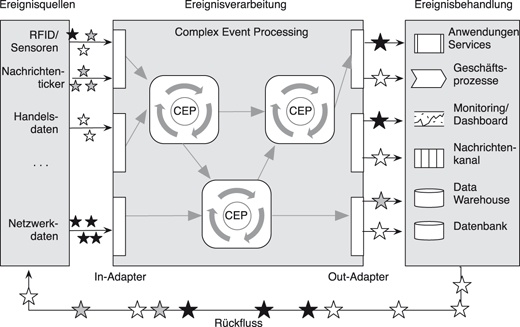
\includegraphics[width=\linewidth]{img/eda-struktur-bruns.jpg}
    \caption{\textit{EDA}-Struktur}
    \label{img:eda-struktur}
\end{figure}

\textit{CEP} ist in erste Linie als Sammelbezeichnung für verschiedene Paradigmen und 
Techniken für die Analyse und Verarbeitung von Ereignissen zu verstehen. Ziel ist es 
Wissen aus einer kontinuierlich nachströmenden Menge an Daten in Form von Ereignissen zu 
generieren. Dies geschieht zum Beispiel durch Korrelation oder Gruppierung von 
Ereignissen nach vorher definierten Regeln. Dabei kann eine Vielzahl von 
Ereignisquellen (Abbildung \ref{img:eda-struktur}) existieren, welche fortlaufend neue 
Ereignisse generieren. Trifft eine Regel auf eine Menge an Ereignissen zu, so wird daraus 
ein komplexes Ereignis (\cite{glossary}) generiert, welches abermals als atomares 
Ereignis für eine weitere 
\textit{CEP}-Instanz dienen kann. Ein komplexes Ereignis wird auch verwendet
um verschiedenartige Meldungen zu generieren, Prozesse zu initiieren oder um als 
Grundlage 
für Visualisierungen zu dienen. In \cite{bruns} wird ein Grundzyklus für 
ereignisgesteuerte Systeme identifiziert (Abbildung \ref{img:cep-zyklus}), der aus den 
drei Schritten Erkennen, Reagieren und Verarbeiten besteht.

\begin{figure}[H]
    \centering
    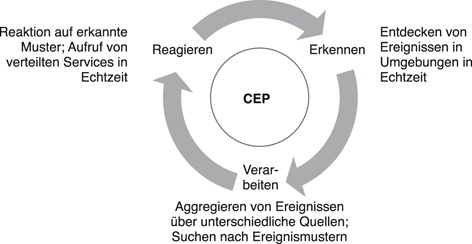
\includegraphics[width=\linewidth]{img/cep-zyklus-bruns.jpg}
    \caption{\textit{CEP}-Zyklus}
    \label{img:cep-zyklus}
\end{figure}

Den Beginn stellt dabei das \emph{Erkennen} dar, relevante Informationen (zum Beispiel 
Messwerte) werden ohne Verzögerung als Ereignisse interpretiert. Während der 
\emph{Verarbeitung} wird die Mustererkennung auf einen oder mehreren Ereignisströmen 
durchgeführt. Sobald Muster erkannt werden, \emph{Reagiert} man mit Meldungen oder mit 
der Generierung komplexer Ereignisse.\\
Laut \cite{eckert} gibt es zwei grundlegende Arten um 
komplexe Ereignisse zu identifizieren. Entweder über bereits bekannte Muster, die durch 
Regeln in Ereignisanfragesprachen formuliert werden können, oder über unbekannte Muster. 
Letztere benötigt allerdings Technologien wie \textit{MachineLearning} und 
\textit{DataMining}, daher wird in diesem Papier nicht darauf eingegangen.

\subsubsection{Begriffsbestimmungen}\label{begriffsbestimmung}
\vspace{0.1cm}
\textbf{\textit{Datenströme/Ereignisströme}}
sind kontinuierliche, kleinteilige Datensätze in der 
zeitlichen Reihenfolge ihres Auftretens oder ihrer Messung. Die Daten weisen eine geringe 
Komplexität auf und beziehen sich nur auf ein Datum (zum Beispiel den Messwert eines 
Sensors oder den Kurs eines Wertpapiers.). Die Ströme sind sind endlos und meist 
hochfrequent und massiv, daher können die Daten nicht persistent gespeichert werden.\\
Jeder Datensatz in einem Datenstrom bildet ein eigenes 
\textbf{\textit{Ereignisse}}. Im 
Allgemeinen kann laut \cite{glossary} ein Ereignis alles sein was eintreten kann, wie zum 
Beispiel ein Erdbeben, eine Finanztransaktion, das Betätigen einer Taste oder die 
Oktoberrevolution. Im speziellen ist ein Ereignis ein aufbereiteter Datensatz, welcher 
die Informationen eines Ereignisses beinhaltet und für die rechnergestützte Verarbeitung 
angepasst ist. Dazu ist es notwendig, dass zum Informationsgehalt des Ereignisses (den 
Kontextinformationen) auch eindeutige und strukturierte Metadaten erfasst werden. 
Exemplarisch 
kann ein Ereignis folgendermaßen aufgebaut sein (\cite{hedtstuck}):

\begin{table}[ht]
    \caption{Ereignisaufbau}
    \label{table:ereignis}\vspace{0.2cm}
    \centering{
        \renewcommand{\arraystretch}{1.3}
        \begin{tabular}{|l|c|}
            \hline
            \multicolumn{2}{|l|}{\cellcolor{shadecolor}\textbf{Metadaten}}\\
            \hline
            Ereignistyp\hspace{0.5cm} &   \texttt{Kursänderung}\\ 
            \hline
            Ereignisquelle\hspace{0.5cm} &   \texttt{Frankfurt}\\ 
            \hline 
            Zeitstempel &   \texttt{2018-11-21 22:14:00}\\
            \hline
            ID          &   \texttt{98127634}\\  
            \hline
            \multicolumn{2}{|l|}{\cellcolor{shadecolor}\textbf{Kontextinformation}}\\     
            \hline
            \multicolumn{2}{|l|}{\texttt{Name: acme GmbH}}\\
            \multicolumn{2}{|l|}{\texttt{Einkaufkurs: 32.5}}\\
            \multicolumn{2}{|l|}{\texttt{Letzer Kurs: 40.8}}\\
            \multicolumn{2}{|l|}{\texttt{Differenzbetrag: 5.7}}\\
            \multicolumn{2}{|l|}{\texttt{Aktualler Kurs: 42.1}}\\
            \hline
        \end{tabular} 
    }
\end{table}
Wobei die Felder \textit{Ereignistyp} und \textit{Ereignisquelle} nach \cite{bruns} 
optional sind. Wie man an den Metainformationen erkennen kann, stehen alle Ereignisse in 
impliziter Beziehung zueinander.\\
Im Verarbeitungsschritt (Abbildung \ref{img:cep-zyklus}) werden Beziehungen zwischen 
Ereignissen gesucht, diese werden durch \textbf{\textit{Ereignismuster}} beschrieben. Die 
Mustererkennung wird nur über einem bestimmtes Zeitintervall des Ereignisstromes 
ausgeführt und durch Ereignisanfragesprachen definiert. In \cite{bruns} werden drei Arten 
von Ereignismustern unterschieden. Können Muster ausschließlich durch boolesche 
Operatoren der Aussagelogik festgelegt werden, so fallen sie in die Kategorie der 
\textit{einfachen Ereignismuster}. Werden hingegen speziellere Operatoren nötig, um zum 
Beispiel die Reihenfolge oder Zeitfenster in den Ereignisse auftreten auszudrücken, 
gehören sie zur Kategorie der \textit{komplexen Ereignismuster}. Zur Kategorie der 
\textit{Abstrakten Ereignismuster} gehören die Muster, welche aus einem bereits erkannten 
Muster komplexe Ereignisse erzeugt um diese auf einer höheren Abstraktionsebene wieder 
zur Verfügung zu stellen.\\
Ein \textbf{\textit{Komplexes Ereignis}} ist eine Menge von Ereignissen, die durch ein 
Ereignismuster beschrieben sind.\\\label{begriff-ereignisregel}
\textbf{\textit{Ereignisregeln}} sind die syntaktische Abstraktion von Ereignismustern 
und werden mithilfe einer \textbf{\textit{Anfragesprache}} erstellt, laut \cite{bruns} 
existieren für diese 
Sprachen kein einheitlicher Standard. Daher existiert eine Fülle an Sprachen, die aber 
alle einige Eigenschaften Teilen. So bestehen alle in einer Anfragesprache formulierten 
Regeln aus einer Prämisse und einem Aktionsteil, wenn das Muster, Beziehungsweise die 
Bedingung in der Prämisse erfüllt ist, wird der Aktionsteil ausgeführt. Anfragesprachen 
sind grundsätzlich deklarativ, man beschreibt also ein Modell und muss keine Verfahren 
zur Mustererkennung implementieren. In \cite{eckert} werden auch reaktive Regeln erwähnt, 
diese Regeln definieren, wie auf komplexe Ereignisse reagiert werden soll.

\subsubsection{Beispielanwendungen}
\vspace{0.1cm}

\textbf{TBD!} wo wird und kann CEP eingesetzt werden\\


%
% Anfragesprachen
%
\subsection{Anfragesprachen}
\vspace{0.1cm}
Mithilfe von Ereignisanfragesprachen lassen sich Daten aus einer Ereignisfolge, eine 
endliche Menge an Ereignissen innerhalb des endlosen Ereignisstromes, extrahieren, 
Ereignisse verdichten, zeitliche zusammenhänge herstellen und Reaktionen festlegen.

\subsubsection{Algebren von Anfragesprachen}
\vspace{0.1cm}
In diesem Abschnitt wird eine Übersicht über die zur Verfügung stehenden Mengenalgebren 
in Anfragesprachen gegeben, dabei wird sich auf das Vorgehen in \cite{bruns} berufen.\\
Seien $A,B,C$ Ereignistypen und $a,b,c$ zugehörige Ereignisinstanzen, wobei gilt 
$a \in A$, $b \in B$ und $c \in C$. Eine Ereignisfolge wird durch $a_1a_2a_3b_1c_1b_21_4$
beschrieben.\\
Jede Ereignisalgebra enthält spezielle Operatoren, die auf Ereignisfolgen angewendet 
werden können und dabei z.B. zeitliche, kausale oder fachliche Zusammenhänge zwischen 
Ereignissen beschreiben. In \textbf{\textit{ereignistypbasierten Mustern}} legt der 
Sequenzoperator die zeitliche Reihenfolge des Auftretens von Ereignistypen fest. Zum 
Beispiel $A \rightarrow B$. Diese Regel akzeptiert die Ereignisfolge $c_1a_1a_2c_2b_1$. 
Des Weiteren existieren die boolesche Operatoren $\land , \lor$, die keine Reihenfolge 
des Auftretens beschreiben, da das Kommutativgesetz gilt: $A \circ B = B \circ A, \circ 
\in {\lor,\land}$. Ebenso existiert die Negation: $\neg A$. Die Kombination dieser 
Operatoren ermöglicht es komplexe Muster in Ereignisfolgen zu erkennen.\\
Eine weitere Algebra, welche von Anfragesprachen implementiert wird, ist die Algebra über 
\textbf{\textit{Kontextbedingungen}}. Mithilfe dieser Algebra ist es möglich direkt 
auf Attribute der Ereignisinstanzen über den $.$-Operator zugreifen zu können. Damit 
besteht die Möglichkeit die Attribute in Relation zu setzen Rechenvorschriften zu 
definieren. Zur Verfügung stehen dabei die numerischen Operatoren und 
Vergleichsoperatoren, aber auch Operatoren für Zeichenketten sind denkbar, oder gesondert 
definierte Methoden. 



%
% ESPER
%
\subsection{Esper}
\vspace{0.1cm}
\subsubsection{Einordnung/Vorstellung  von Esper}
\vspace{0.1cm}
\subsubsection{Funktionalität von Esper}
\vspace{0.1cm}
\subsubsection{Anfragesprache EPL}
\vspace{0.1cm}

%
% Problembeispiel
%

\subsection{Problembeispiel mit Esper}
\vspace{0.1cm}
\subsubsection{Problembeschreibung}
\vspace{0.1cm}
\subsubsection{Implementierung mit Esper}
\vspace{0.1cm}
\subsubsection{Ergebnis}
\vspace{0.1cm}


%
% Schlussfolgerung
%

\section{Schlussfolgerung}
\vspace{0.1cm}

%\section{Danksagung}
%Vielen Dank an die Entwickler von Esper und die gute Dokumentation der Software.\\

\appendix
\vspace{0.1cm}
%
% The following two commands are all you need in the
% initial runs of your .tex file to
% produce the bibliography for the citations in your paper.
\bibliographystyle{abbrv}
\bibliography{bib/bibo}  % sigproc.bib is the name of the Bibliography in this case
% You must have a proper ".bib" file
%  and remember to run:
% latex bibtex latex latex
% to resolve all references
%
% ACM needs 'a single self-contained file'!
%
%APPENDICES are optional
%\balancecolumns

%Appendix A


\end{document}
